\documentclass[varwidth=true, border=2pt]{standalone}

\usepackage{pgfplots}
\usepackage{tikz}

\usetikzlibrary{calc,patterns,angles,quotes}

\begin{document}
	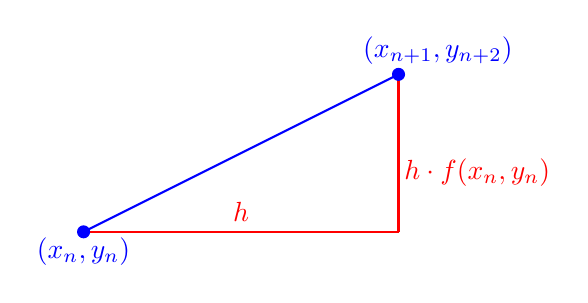
\begin{tikzpicture}
	\node (O) at (0,0) {};
	\node (B) at (4,0) {};
	\node (C) at (4,2) {};
	\node [red](RUN) at (2,0.25) {$h$};
	\node [red](RISe) at (5,0.75) {$h \cdot f(x_n,y_n)$};
	\node [blue](O1) at (0,-0.25){($x_n,y_n)$};
	\node [blue](C1) at (4.5,2.3){($x_{n+1},y_{n+2})$};
 	  
	\draw [thick,red] (O.center) to (B.center);
	\draw [thick,blue] (O.center) to (C.center);
	\draw [thick,red] (B.center) to (C.center);

	\draw[blue,fill=blue] (0,0) circle (.5ex);
	\draw[blue,fill=blue] (4,2) circle (.5ex);
	\end{tikzpicture}
\end{document}